\documentclass{IEEEtran}

\usepackage{amsmath}
\usepackage{graphicx}
\usepackage{tfrupee}

\title{Assignment I - ICSE 10 2018 - Q9(a)}
\author{Kartheek Tammana}

\begin{document}
\maketitle

The various parameters given are listed in the following table:

\begin{center}
\begin{tabular}{|l|l|l|}
    \hline
    Symbol & Description & Value \\
    \hline
    $I$ & Interest & \rupee 5550 \\
    $P$ & Monthly Deposit & \rupee 1000 \\
    $r$ & Annual Interest Percentage & 10\% \\
    $n$ & Number of Months & ? \\
    \hline
\end{tabular}
\end{center}

We know the formula for interest on a recurring deposit is:
\begin{align}
    I &= \frac{P \cdot n(n+1) \cdot r}{12 \cdot 2 \cdot 100} \\
    \implies 5550 &= \frac{1000 \cdot n(n+1) \cdot 10}{12 \cdot 2 \cdot 100} \\
    \implies n(n+1) &= 1332 \\
                    &= 36 \cdot 37
\end{align}
Solving the quadratic, we get $n=36$ or $n=-37$. Discarding the negative solution, we get that the
time of maturity is 36 months, or 3 years. \\ \\
We can verify this answer by graphing the interest as a function of time, i.e.,
\begin{equation}
    y = \frac{1000 \cdot x(x+1) \cdot 10}{12 \cdot 2 \cdot 100}
\end{equation}
along with the interest at time of maturity $y=5550$, and checking for the point of intersection,
where $y$ is the interest in rupees, and $x$ is time in months.

\centering
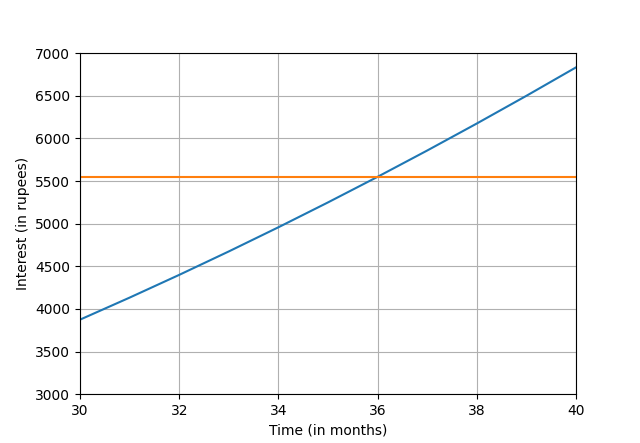
\includegraphics[width=0.75\columnwidth]{./figs/fig.png}
\end{document}
